\documentclass{article}
\usepackage{graphicx} % Required for inserting images
% --- Packages for Higher Mathematics ---
\usepackage{amsmath, amsfonts, amssymb, amsthm} % Standard AMS math suite
\usepackage{enumitem}                          % Better lists for problem sets
\usepackage{caption}
% --- Theorem & Proof Environments ---
\theoremstyle{definition}
\newtheorem{problem}{Problem}
% Custom Solution Environment
\newenvironment{solution}
  {\par\vspace{0.5em}\noindent\textbf{Solution:}\par\nopagebreak\vspace{0.3em}}
  {\par\vspace{1em}}
\usepackage[
  top=0.2in,
  bottom=0.1in,
  left=0.25in,
  right=1in
]{geometry}
\usepackage{tikz}
\usetikzlibrary{
  calc,                  % Coordinate math: ($(A)!0.5!(B)$)
  patterns,              % Surface hatching (ground, walls)
  decorations.pathmorphing, % Springs, zigzags
  decorations.markings,  % Arrows along paths (magnetic fields, rays)
  angles, quotes         % Easy angle arc marking
}
\usetikzlibrary{arrows.meta}
\usepackage{multicol} % Load the package
\title{Statics Solutions}
\author{Sanay Pathak}
\date{August 2026}

\begin{document}
\maketitle
\begin{problem}
    \begin{minipage}[t]{0.95\textwidth}
        A person pulls on a block with a force $F$, at an angle $\theta$ with respect to the horizontal. The coefficient of friction between the block and the ground is $\mu$.
        For what $\theta$ is the $F$ required to make the block slip a minimum?
    \end{minipage}
\end{problem}
\begin{solution}
\noindent
\begin{minipage}[t]{0.90\textwidth}
  \vspace{0pt}
  \begin{tabular}{@{}p{0.5\textwidth} p{0.5\textwidth}@{}}
    Horizontally, & Vertically, \\
    $\begin{aligned}
        &F \cos \theta = \mu N \\
        \implies &N = \frac{F \cos \theta}{\mu} \quad (1)
    \end{aligned}$ 
    & 
    $\begin{aligned}
        &F \sin \theta + N = Mg \\
        \implies &N = Mg - F \sin \theta \quad (2)
    \end{aligned}$
  \end{tabular}

  \vspace{1em}
  Equating (1) and (2),
  \begin{align*}
      &F \cos \theta = \mu Mg - \mu F \sin \theta \\
      \implies &F = \frac{\mu Mg}{\cos \theta + \mu \sin \theta}
  \end{align*}

  Now to reduce $F$, we must maximize $\cos \theta + \mu \sin \theta$. Differentiating and equating to $0$, we get:
  \begin{align*}
      &-\sin \theta + \mu \cos \theta = 0\\
      \implies &\tan \theta = \mu \\
      \implies &\theta = \tan^{-1}\mu
  \end{align*}
\end{minipage}%
\hfill
\begin{minipage}[t]{0.10\textwidth}
  \vspace{0pt}
  \centering
  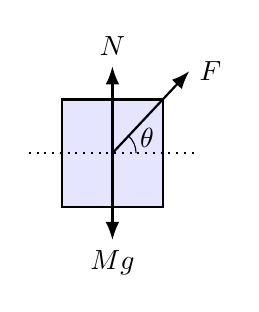
\begin{tikzpicture}[scale=0.85]
      \draw[thick, fill=blue!10] (2.5,0) rectangle (4,1.6);
      \draw[-Latex, thick, black] (3.25, 0.8) -- (3.25, -0.5) node[below] {$Mg$};
      \draw[-Latex, thick, black] (3.25, 0.8) -- (3.25, 2.1) node[above] {$N$};
      \draw[-Latex, thick, black] (3.25, 0.8) -- (4.4, 2.02667) node[right] {$F$};
      \draw[dotted, thick] (2,0.8) -- (4.5,0.8);
      
      \coordinate (A) at (4.4, 2.02667);
      \coordinate (B) at (3.25, 0.8);
      \coordinate (C) at (4.5, 0.8);
      \pic [draw, "$\theta$", angle radius=0.3cm, angle eccentricity=1.6] {angle = C--B--A};
  \end{tikzpicture}
\end{minipage}
\end{solution}
\newpage
\begin{problem}
    \noindent
    \begin{minipage}[c]{0.66\textwidth}
        \begin{enumerate}[label=(\alph*), leftmargin=*]
            \item Consider the first bridge in Fig.~1, made of three equilateral triangles of beams. Assume that the seven beams are massless and that the connection between any two of them is a hinge. If a car of mass $m$ is located at the middle of the bridge, find the forces (and specify tension or compression) in the beams. Assume that the supports provide no horizontal forces on the bridge.
            \item Same question, but now with the second bridge in Fig.~1, made of seven equilateral triangles.
            \item Same question, but now with the general case of $4n-1$ equilateral triangles.
        \end{enumerate}
    \end{minipage}%
    \hfill
    \begin{minipage}[c]{0.20\textwidth}
        \centering
        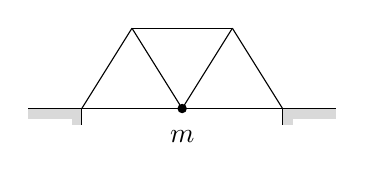
\begin{tikzpicture}[scale=0.85]
            \draw (-0.8,0) -- (0,0);
            \draw (3,0) -- (3.8,0);
            \fill[gray!30] (-0.8,0) rectangle (0,-0.15);
            \fill[gray!30] (3,0) rectangle (3.8,-0.15);
            \fill[gray!30] (0,0) rectangle (-0.15,-0.25);
            \fill[gray!30] (3,0) rectangle (3.15,-0.25);
            \draw (0,0) -- (0,-0.25);
            \draw (3,0) -- (3,-0.25);
            \draw (0,0) -- (3,0);
            \draw (0.75,1.2) -- (2.25,1.2);
            \draw (0,0) -- (0.75,1.2);
            \draw (0.75,1.2) -- (1.5,0);
            \draw (1.5,0) -- (2.25,1.2);
            \draw (2.25,1.2) -- (3,0);
            \fill (1.5,0) circle (2pt);
            \node at (1.5,-0.42) {$m$};
        \end{tikzpicture}
        
        \vspace{0.3cm}
        
        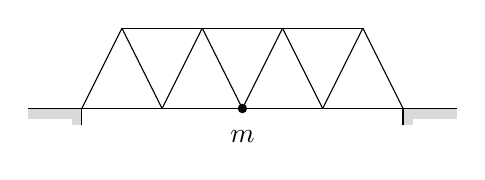
\begin{tikzpicture}[scale=0.85]
            \draw (-0.8,0) -- (0,0);
            \draw (4.8,0) -- (5.6,0);
            \fill[gray!30] (-0.8,0) rectangle (0,-0.15);
            \fill[gray!30] (0,0) rectangle (-0.15,-0.25);
            \fill[gray!30] (4.8,0) rectangle (5.6,-0.15);
            \fill[gray!30] (4.8,0) rectangle (4.95,-0.25);
            \draw (0,0) -- (0,-0.25);
            \draw (4.8,0) -- (4.8,-0.25);
            \draw (0,0) -- (0,-0.25);
            \draw (0,0) -- (4.8,0);
            \draw (0.6,1.2) -- (4.2,1.2);
            \draw (0,0) -- (0.6,1.2);
            \draw (0.6,1.2) -- (1.2,0);
            \draw (1.2,0) -- (1.8,1.2);
            \draw (1.8,1.2) -- (2.4,0);
            \draw (2.4,0) -- (3.0,1.2);
            \draw (3.0,1.2) -- (3.6,0);
            \draw (3.6,0) -- (4.2,1.2);
            \draw (4.2,1.2) -- (4.8,0);    
            \fill (2.4,0) circle (2pt);
            \node at (2.4,-0.42) {$m$};
        \end{tikzpicture}
        \captionof{figure}{}
        \label{fig:1}
    \end{minipage}
\end{problem}
\begin{solution}
    \noindent
    \begin{minipage}[c]{0.85\textwidth}
      \vspace{0pt}
      We solve only for $4n-1$ triangles. The previous two cases can simply be substituted in the formula. Since the figure is symmetrical, the mass at center will be balanced equally from both supports each providing an upward force of $\frac{mg}{2}$.
      \\Therefore, at A, vertically,
      \\
      \begin{align*}
          &F_{AB} \sin 60^\circ +\frac{mg}{2} = 0
          \\ \implies &F_{AB}=- \frac{mg}{\sqrt{3}}
      \end{align*}
      \\Horizontally
      \begin{align*}
          &F_{AB} \cos 60^\circ +F_{AC} = 0
          \\ \implies &F_{AC}= \frac{mg}{2\sqrt{3}} 
      \end{align*}
      \\
      \\Now, at B, vertically,
      \begin{align*}
          &F_{AB} \sin 60^\circ +F_{BC}\sin 60^\circ = 0
          \\ \implies &F_{BC}= \frac{mg}{\sqrt{3}} 
      \end{align*}
      Based on this we can say, all diagonals have alternatively same force of compression and tension.
      \\Horizontally, 
      \begin{align*}
          &F_{AB} \cos 60^\circ +F_{BC}\cos 60^\circ = F_{BD}
          \\ \implies &F_{BD}= \frac{mg}{\sqrt{3}}
      \end{align*}
      \\
      \\Now, at $CE$, there is an extra force of $AC$ plus an extra force due to tension of $BC$ aside from the arrangement that like the previous. Hence 
      $$F_{extra}=\frac{mg}{ \sqrt{3}} $$
      Therefore, $F_{CE}=\frac{3mg}{ 2\sqrt{3}}$. Similarly continuously, adding $F_{extra}=\frac{mg}{ \sqrt{3}} $ for subsequent chords, upto the center we arrive at the center,
      $$F_{bottom}=\frac{(2k-1) mg}{ 2\sqrt{3}}$$  where $k \in \{1, 2, \dots, n\}$ denotes the index of the bottom chord section counted from the outer support towards the center.
      \\\\Similarly for the top chord, at every junction, an extra $\frac{mg}{\sqrt{3}}$ is added. so it comes $$F_{top}=\frac{p mg}{ 2\sqrt{3}}$$ where $p \in \{1, 2, \dots, n\}$ denotes the index of the top chord section counted from the outer support towards the center.
    \end{minipage}%
    \hfill
    \begin{minipage}[c]{0.15\textwidth}
      \vspace{0pt}
        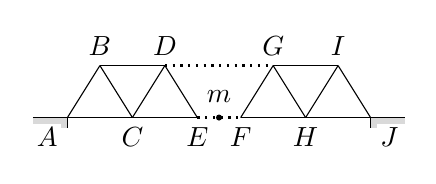
\begin{tikzpicture}[scale=0.55]
            \draw (-0.8,0) -- (0,0);
            \fill[gray!30] (-0.8,0) rectangle (0,-0.15);
            \fill[gray!30] (0,0) rectangle (-0.15,-0.25);
            \draw (0,0) -- (0,-0.25);
            \draw (0,0) -- (3,0);
            \draw (0.75,1.2) -- (2.25,1.2);
            \draw (0,0) -- (0.75,1.2);
            \draw (0.75,1.2) -- (1.5,0);
            \draw (1.5,0) -- (2.25,1.2);
            \draw (2.25,1.2) -- (3,0);
            \draw[dotted, thick] (3,0) -- (4,0);
            \draw[dotted, thick] (2.25,1.2) -- (4.75,1.2);
            \draw (4,0) -- (7,0);
            \draw (4.75,1.2) -- (6.25,1.2);
            \draw (4,0) -- (4.75,1.2);
            \draw (4.75,1.2) -- (5.5,0);
            \draw (5.5,0) -- (6.25,1.2);
            \draw (6.25,1.2) -- (7,0);
            \fill (3.5,0) circle (2pt);
            \node[anchor=south] at (3.5,0.12) {$m$};
            \draw (7,0) -- (7.8,0);
            \fill[gray!30] (7,0) rectangle (7.8,-0.15);
            \fill[gray!30] (7,0) rectangle (7.15,-0.25);
            \draw (7,0) -- (7,-0.25);
            \node[anchor=north east] at (0,0) {$A$};
            \node[anchor=south] at (0.75,1.2) {$B$};
            \node[anchor=north] at (1.5,0) {$C$};
            \node[anchor=south] at (2.25,1.2) {$D$};
            \node[anchor=north] at (3,0) {$E$};
            
            \node[anchor=north] at (4,0) {$F$};
            \node[anchor=south] at (4.75,1.2) {$G$};
            \node[anchor=north] at (5.5,0) {$H$};
            \node[anchor=south] at (6.25,1.2) {$I$};
            \node[anchor=north west] at (7,0) {$J$};
        \end{tikzpicture}
    \end{minipage}
\end{solution}
\begin{problem}
    \begin{minipage}[c]{0.66\textwidth}
        A rope rests on two platforms that are both inclined at an angle $\theta$ (which you are free to pick), as shown in Fig. 2. The rope has uniform mass density, and its coefficient of friction with the platforms is 1. The system has left-right symmetry. What is the largest possible fraction of the rope that does not touch the platforms? What angle $\theta$ allows this maximum value?
    \end{minipage}
    \hfill
    \begin{minipage}[c]{0.30\textwidth}
        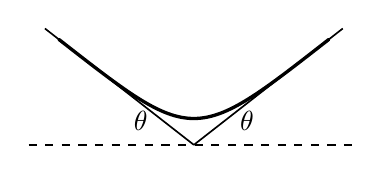
\begin{tikzpicture}[scale=1.5]
          \def\angle{38}       % Angle theta in degrees
          \def\rBase{1.6}      % Length of thin outer guide lines
          \def\rContact{1.45}  % Contact/tangency point distance from vertex
          \def\rThick{1.45}    % Upper end of thick line
          \coordinate (V) at (0,0);
          \path (V) ++(180-\angle:\rBase) coordinate (L_end);
          \path (V) ++(\angle:\rBase) coordinate (R_end);
          \path (V) ++(180-\angle:\rContact) coordinate (P_L);
          \path (V) ++(\angle:\rContact) coordinate (P_R);
          \path (V) ++(180-\angle:\rThick) coordinate (T_L);
          \path (V) ++(\angle:\rThick) coordinate (T_R);
          \draw[dashed, line width=0.6pt] (-1.4, 0) -- (1.4, 0);
          \draw[line width=0.6pt] (V) -- (L_end);
          \draw[line width=0.6pt] (V) -- (R_end);
          \draw[line width=1.2pt, line cap=round] (T_L) -- (P_L) .. controls (V) .. (P_R) -- (T_R);
          \node at (-0.45, 0.2) {$\theta$};
          \node at (0.45, 0.2) {$\theta$};
        \end{tikzpicture}
        \captionof{figure}{}
    \end{minipage}
\end{problem}
\begin{solution}
    Let $f$ be the fraction of the wire hanging.  
    Therefore, $\frac{1-f}{2}$ fraction is on each side of the rod.
    
    Let tension $T$ act at the base angle $\theta$.  
    Mass of the hanging portion = $\rho f$.
    
    Balancing forces on the hanging portion:
    $$2T \sin\theta = \rho f g$$
    
    For the wire segment resting on the rod:
    $$mg \sin\theta + T = mg \cos\theta$$
    
    Substituting $m = \rho \left(\frac{1-f}{2}\right)$:
    \begin{align*}
        \rho \left(\frac{1-f}{2}\right) g \sin\theta + T &= \rho \left(\frac{1-f}{2}\right) g \cos\theta \\
        \implies T &= \left(\frac{1-f}{2}\right) \rho g (\cos\theta - \sin\theta)
    \end{align*}
    
    Substituting $T$ into the force-balance equation:
    \begin{align*}
        2\left(\frac{1-f}{2}\right) \rho g (\cos\theta - \sin\theta) \sin\theta &= \rho f g \\
        \implies \frac{1-f}{f} &= \frac{1}{(\cos\theta - \sin\theta) \sin\theta} \\
        \implies \frac{1}{f} &= \frac{1}{\sin\theta \cos\theta - \sin^2\theta} + 1 \\
        \implies \frac{1}{f} &= \frac{\sin\theta \cos\theta + \cos^2\theta}{\sin\theta \cos\theta - \sin^2\theta} \\
        \implies f &= \frac{\sin\theta}{\cos\theta} \left[ \frac{\cos\theta - \sin\theta}{\cos\theta + \sin\theta} \right] \\
        \implies f &= \tan\theta \left[ \frac{1 - \tan\theta}{1 + \tan\theta} \right]
    \end{align*}

    To maximize $f(\theta)$, let $x = \tan\theta$:
    \begin{align*}
        f &= \frac{x - x^2}{1 + x} \\
        f' &= \frac{(1 - 2x)(1 + x) - (x - x^2)(1)}{(1 + x)^2} = 0 \\
        \implies 1 - 2x - 2x^2 - x + x^2 &= 0 \\
        \implies -x^2 - 2x + 1 &= 0 \\
        \implies x^2 + 2x - 1 &= 0 \\
        \implies x &= \sqrt{2} - 1
    \end{align*}
    
    $$\text{Optimal angle } \implies \theta = \tan^{-1}(\sqrt{2} - 1) = \frac{\pi}{8} = 22.5^\circ$$
    
    Calculating the maximum fraction:
    \begin{align*}
        \text{Maximum fraction} &= \frac{x(1 - x)}{1 + x} \\
        &= \frac{(\sqrt{2} - 1)(2 - \sqrt{2})}{\sqrt{2}} \\
        &= \frac{2\sqrt{2} - 2 - 2 + \sqrt{2}}{\sqrt{2}} \\
        &= \frac{3\sqrt{2} - 4}{\sqrt{2}} \\
        &= \frac{6 - 4\sqrt{2}}{2} \\
        &= 3 - 2\sqrt{2}
    \end{align*}
\end{solution}
\begin{problem}
    \begin{minipage}[c]{0.66\textwidth}
        A chain of mass $M$ hangs between two walls, with its ends at the same height. The chain makes an angle of $\theta$ with each wall, as shown in Fig.~1.11. Find the tension in the chain at the lowest point. Solve this by:
        \begin{enumerate}
            \item[(a)] Considering the forces on half of the chain. (This is the quick way.)
            \item[(b)] Using the fact that the height of a hanging chain is given by $y(x) = \frac{1}{\alpha}\cosh(\alpha x)$, and considering the vertical forces on an infinitesimal piece at the bottom. (This is the long way.)
        \end{enumerate}
    \end{minipage}
    \hfill
    \begin{minipage}[c]{0.30\textwidth}
        \centering
        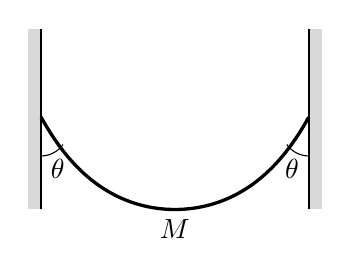
\begin{tikzpicture}[scale=0.85]
            \fill[gray!30] (-2.2, -0.5) rectangle (-2, 2.2);
            \draw[line width=0.8pt] (-2, -0.5) -- (-2, 2.2);
            \fill[gray!30] (2, -0.5) rectangle (2.2, 2.2);
            \draw[line width=0.8pt] (2, -0.5) -- (2, 2.2);
            \draw[line width=1.2pt] plot[domain=-2:2, samples=100] (\x, {0.5*cosh(\x) - 1.0});
            \draw (-2, 0.3) arc (-90:-35:0.4);
            \node at (-1.75, 0.1) {$\theta$};
            \draw (2, 0.3) arc (-90:-145:0.4);
            \node at (1.75, 0.1) {$\theta$};
            \node[below] at (0, -0.5) {$M$};
        \end{tikzpicture}
        \captionof{figure}{}
    \end{minipage}
\end{problem}
\begin{solution}
    \begin{enumerate}
        \item[\textbf{(a)}] \textbf{At the top}

        \noindent
        \begin{minipage}[t]{0.62\textwidth}
            \vspace{0pt}
            Taking half the chain (it can be done since the figure is symmetric).

            Balancing weight of half chain:
            \begin{align*}
                T \cos \theta &= \frac{M}{2} g
            \end{align*}

            Balancing horizontally:
            \begin{align*}
                T' &= T \sin \theta \\
                \implies T' &= \frac{M}{2} g \frac{\sin \theta}{\cos \theta} = \frac{Mg}{2} \tan \theta
            \end{align*}
        \end{minipage}%
        \hfill
        \begin{minipage}[t]{0.32\textwidth}
            \vspace{0pt}
            \centering
            \begin{tikzpicture}[scale=1.0]
                % Curve representing half chain
                \draw[thick] (0,0) parabola (2,2.5);
                
                % Tick mark at bottom
                \draw (0,-0.15) -- (0,0.15);
                
                % Horizontal tension T' pointing left
                \draw[thick, <-] (-1,0) -- (0,0) node[below, pos=0.2] {$T'$};
                
                % Vertical reference line at the top
                \draw[thick] (2,0) -- (2,3.2);
                
                % Tangent Vector T at the top
                \draw[thick, ->] (2,2.5) -- (2.3, 3.2) node[right] {$T$};
                
                % Angle theta
                \draw (2,2.9) arc (90:66:0.4);
                \node at (2.12,3.05) {$\theta$};
            \end{tikzpicture}
        \end{minipage}

        \vspace{1em}

        \item[\textbf{(b)}] For any infinitesimal piece at any point,

        \noindent
            \vspace{0pt}
            Since tension is tangential,
            \begin{align*}
                \frac{T_y}{T_x} &= \tan \theta = \frac{dy}{dx}
            \end{align*}

            Now, since no external force is applied, $T_x$ is constant throughout.
        

        Now balancing mass:
        \begin{align*}
            dm \, g &= d T_y \\
                    &= d \left( T_x \frac{dy}{dx} \right)
        \end{align*}

        Given:
        \begin{align*}
            y &= \frac{1}{\alpha} \cosh(\alpha x) \\
            \frac{dy}{dx} &= \frac{\alpha}{\alpha} \sinh(\alpha x) = \sinh(\alpha x)
        \end{align*}

        Now arc length $ds$:
        \begin{align*}
            ds &= \sqrt{(dx)^2 + (dy)^2} \\
               &= \sqrt{1 + {y'}^2} \, dx \\
               &= \sqrt{1 + \sinh^2(\alpha x)} \, dx \\
               &= \cosh(\alpha x) \, dx
        \end{align*}

        Equating mass/force balance:
        \begin{align*}
            \cosh(\alpha x) \, dx \cdot \lambda g &= d(T_x \sinh(\alpha x)) = \alpha T_x \cosh(\alpha x) \, dx \\
            \implies \alpha T_x &= \lambda g \\
            \implies \alpha &= \frac{\lambda g}{T_x}
        \end{align*}

        At a corner:
        \begin{align*}
            \sinh(\alpha x_0) &= \cot \theta
        \end{align*}

        Now total mass:
        \begin{align*}
            \int dm &= \lambda \int ds = \lambda \int_{-x_0}^{x_0} \cosh(\alpha x) \, dx \\
                    &= \frac{\lambda}{\alpha} \Big[ \sinh(\alpha x) \Big]_{-x_0}^{x_0} = \frac{2\lambda}{\alpha} \sinh(\alpha x_0)
        \end{align*}
        Now,
        \begin{align*}
            M &= \frac{2\lambda}{\alpha} \sinh(\alpha x_0) \\
              &= \frac{2\lambda \cot\theta \, T_x}{\lambda g} \\[0.5em]
            Mg &= 2 T_x \cot\theta \\
            \implies T_x &= \frac{Mg}{2 \cot\theta} \\
                         &= \frac{Mg}{2} \tan\theta
        \end{align*}
    \end{enumerate}
\end{solution}
\begin{problem}
    \begin{minipage}[t]{0.95\textwidth}
        A stick is connected to other parts of a system by hinges at its ends. Show that if the stick is massless, then the forces it feels at the hinges are directed along the stick; but if the stick has mass, then the forces need not point along the stick.
    \end{minipage}
\end{problem}
\begin{solution}
    \text{Since the stick is massless, the moment of inertia comes to be zero.}
    By definition,
    \begin{align*}
    \tau &= I\alpha = 0 \\
    \implies Fd\sin\theta &= 0
    \end{align*}
    If $F \neq 0$ and $d \neq 0$,
    \begin{align*}
    \implies \sin\theta &= 0 \\
    \implies \theta &= 0^\circ
    \end{align*}
    Therefore, the forces are along the stick.
    However, if the stick has mass,
    \begin{align*}
    \tau &= I\alpha \\
    &= a, \qquad a \in \mathbb{R}
    \end{align*}
    \begin{align*}
    \implies \sin\theta &\neq 0
    \end{align*}
    Thus, $\theta$ is not necessarily zero.
\end{solution}
\newpage
\begin{problem}
    A horizontal stick of mass $M$ and length $L$ is pivoted at one end. Integrate the gravitational torque along the stick (relative to the pivot), and show that the result is the same as the torque due to a mass $M$ located at the center of the stick.
\end{problem}
\begin{solution}
    \begin{minipage}[c]{0.45\textwidth}
        \centering
        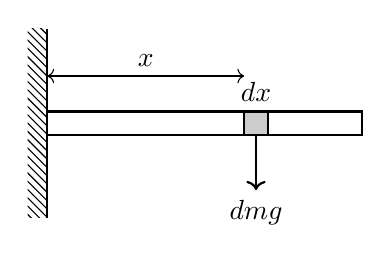
\begin{tikzpicture}[scale=1.0]
    
            % Wall / Support
            \draw[thick] (0, -1.2) -- (0, 1.2);
            \fill[pattern=north west lines] (-0.25, -1.2) rectangle (0, 1.2);
    
            % Rod
            \draw[thick] (0, 0.15) -- (4.0, 0.15) -- (4.0, -0.15) -- (0, -0.15);
    
            % Element dx
            \fill[gray!40] (2.5, -0.15) rectangle (2.8, 0.15);
            \draw[thick] (2.5, -0.15) rectangle (2.8, 0.15);
    
            % Distance x and element dx labels
            \draw[<->] (0, 0.6) -- (2.5, 0.6) node[midway, above] {$x$};
            \node[above] at (2.65, 0.15) {$dx$};
    
            % Arrow pointing down for dm
            \draw[->, thick] (2.65, -0.15) -- (2.65, -0.85);
            \node[below] at (2.65, -0.85) {$dm g$};
        \end{tikzpicture}
    \end{minipage}%
    \hfill
    \begin{minipage}[c]{0.52\textwidth}
    \begin{align*}
    \text{At a distance, } dm &= \lambda dx \cdot g \\
    d\tau &= \lambda dx \cdot x \cdot g \\
    \implies \int_0^{\tau_0} d\tau &= \int_0^L \lambda x dx \cdot g \\
    \implies \tau_0 &= \frac{\lambda L^2}{2} g \qquad \text{Now } \lambda L = M \\
    &= \frac{MgL}{2} \\
    &= (Mg)\left(\frac{L}{2}\right)
    \end{align*}
    \end{minipage}
\end{solution}
\begin{problem}
    \begin{minipage}[c]{0.65\textwidth}
        A ball is held up by a string, as shown in Fig. 4, with the string tangent to the ball. If the angle between the string and the wall is $\theta$, what is the minimum coefficient of static friction between the ball and the wall, if the ball is not to fall?
    \end{minipage}
    \begin{minipage}[c]{0.42\textwidth}
        \centering
        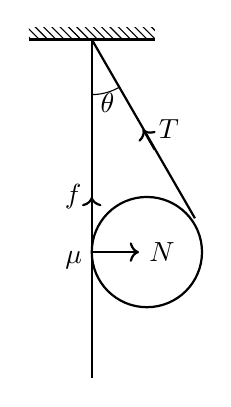
\begin{tikzpicture}[scale=1]

    
            % Ceiling support
            \draw[thick] (-0.8, 2.5) -- (0.8, 2.5);
            \fill[pattern=north west lines] (-0.8, 2.5) rectangle (0.8, 2.65);
    
            % Vertical wall line
            \draw[thick] (0, 2.5) -- (0, -1.8);
    
            % Sphere / Cylinder
            \draw[thick] (0.7, -0.2) circle (0.7);
    
            % Tension string attached to top and tangent to cylinder
            \draw[thick] (0, 2.5) -- (1.31, 0.23);
            
            % Arrow on tension string
            \draw[->, thick] (0.8, 1.1) -- (0.65, 1.36) node[right, xshift=2pt] {$T$};
    
            % Angle theta arc
            \draw (0, 1.8) arc (-90:-60:0.7);
            \node at (0.2, 1.7) {$\theta$};
    
            % Force vectors on the sphere
            % Normal force N
            \draw[->, thick] (0, -0.2) -- (0.6, -0.2) node[right] {$N$};
            
            % Friction force f
            \draw[->, thick] (0, -0.2) -- (0, 0.5) node[left] {$f$};
    
            % Friction coefficient mu
            \node[left] at (0, -0.3) {$\mu$};
        \end{tikzpicture}
        \captionof{figure}{}
    \end{minipage}%
    \hfill
\end{problem}
\begin{solution}
    \begin{align*}
        \text{Now, } N &= T \sin\theta \\
        f &= \mu N = \mu T \sin\theta \\        
        \therefore\text{TR} & \le \mu T \sin\theta \cdot R \\
        \mu &= \csc\theta
    \end{align*}
\end{solution}
\begin{problem}
    You hold one end of a stick of mass $M$ and length $L$. A quarter of the way up the stick, it rests on a frictionless corner of a table. The stick makes an angle $\theta$ with the horizontal. What is the magnitude of the force your hand must apply, to keep the stick in this position? For what angle is the vertical component of your force equal to zero?
\end{problem}
\begin{solution}
    \begin{minipage}[t]{0.42\textwidth}
    \vspace{0pt}
    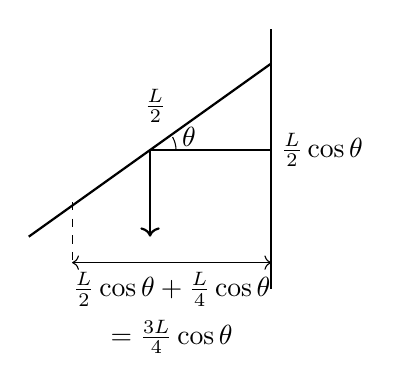
\begin{tikzpicture}[scale=1.1]
        % Vertical wall
        \draw[thick] (2, -1.8) -- (2, 1.2);
        
        % Slanted rod
        \draw[thick] (-0.8, -1.2) -- (2, 0.8);
        
        % Center mark / downward gravity arrow
        \draw[->, thick] (0.6, -0.2) -- (0.6, -1.2);
        
        % Horizontal reference line for angle theta
        \draw (0.6, -0.2) -- (2, -0.2);
        \node[right] at (2, -0.2) {$\frac{L}{2}\cos\theta$};
        
        % Angle arc theta
        \draw (0.9, -0.2) arc (0:30:0.3);
        \node at (1.05, -0.05) {$\theta$};
        
        % Label L/2 along the rod
        \node[above left] at (0.9, 0) {$\frac{L}{2}$};
        
        % Bottom horizontal dimension arrow
        \draw[<->] (-0.3, -1.5) -- (2, -1.5);
        \node[below, align=center] at (0.85, -1.5) {
            $\frac{L}{2}\cos\theta + \frac{L}{4}\cos\theta$ \\[4pt]
            $= \frac{3L}{4}\cos\theta$
        };
        
        % Vertical reference projection line to bottom dimension
        \draw[dashed] (-0.3, -0.8) -- (-0.3, -1.5);
        \draw[dashed] (2, -0.2) -- (2, -1.5);
    \end{tikzpicture}
    \end{minipage}%
    \hfill
    \begin{minipage}[t]{0.55\textwidth}
    \vspace{0pt}
    \textbf{About wall}
    
    \begin{align*}
    Mg \frac{L}{2} \cos\theta &= N \cdot \frac{3L}{4} \cos\theta \\[6pt]
    \implies \frac{2Mg}{3} &= N
    \end{align*}
    
    \end{minipage}
\end{solution}
\begin{problem}
    \begin{minipage}[c]{0.75\textwidth}
        A ladder of mass $M$ and length $L$ leans against a frictionless wall, with a quarter of its length hanging over a corner, as shown in Fig. 5. Assuming that there is sufficient friction at the corner to keep the ladder at rest, what is the total force that the corner exerts on the ladder?
    \end{minipage}
    \begin{minipage}[c]{0.22\textwidth}
        \centering
        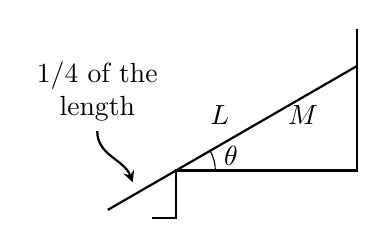
\begin{tikzpicture}[scale=1]
            % Draw solid boundaries of the step
            \draw[thick] (-0.3,-0.6) -- (0,-0.6) -- (0,0) -- (2.3,0) -- (2.3,1.8);
            
            % Draw the ladder/rod (slanted line)
            % Angle is approximately 30 degrees, passes through step corner (0,0)
            % Length is divided into 1/4 (below corner) and 3/4 (above corner)
            \draw[thick] (-0.866, -0.5) -- (2.3, 1.328);
            
            % Angle arc and label theta
            \draw (0.5,0) arc (0:30:0.5);
            \node at (0.7,0.18) {$\theta$};
            
            % Labels for Length (L) and Mass (M)
            \node[above left] at (0.8, 0.46) {$L$};
            \node[above right] at (1.3, 0.46) {$M$};
            
            % Curved arrow pointing to the 1/4 length section
            \draw[stealth-, thick] (-0.55, -0.15) to[out=110, in=-90] (-1.0, 0.5);
            \node[above, align=center] at (-1.0, 0.5) {1/4 of the\\length};
        \end{tikzpicture}
        \captionof{figure}{}
    \end{minipage}%
    \hfill
\end{problem}
\begin{solution}
        \begin{align*}
        \frac{3}{4} M g \frac{3}{4} L \cos\theta &= F_H \frac{L}{4} \cos\theta + \frac{M}{4} g \frac{L}{8} \cos\theta \\
        \left( \frac{3}{4} - \frac{1}{8} \right) g M L &= F_H L \\
        \implies \frac{5}{8} M g &= F_H
        \end{align*}
\end{solution}
\begin{problem}
    Two sticks, each of mass $m$ and length $l$, are connected by a hinge at their top ends. They each make an angle $\theta$ with the vertical. A massless string connects the bottom of the left stick to the right stick, perpendicularly. The whole setup stands on a frictionless table. 
    \begin{enumerate}[label=(\alph*)]
        \item What is the tension in the string?
        \item What force does the left stick exert on the right stick at the hinge? Hint: No messy calculations required!
    \end{enumerate}
\end{problem}
\begin{solution}
    \noindent
    \begin{minipage}[t]{0.35\textwidth}
    \vspace{0pt}
    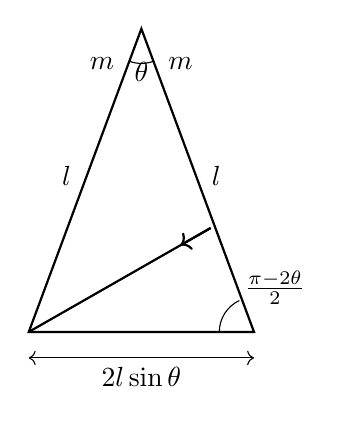
\begin{tikzpicture}[scale=1.1]
        % Main Triangle structure
        \draw[thick] (0,3.5) -- (-1.3,0) -- (1.3,0) -- cycle;
        
        % Base length label
        \draw[<->] (-1.3,-0.3) -- (1.3,-0.3) node[midway, below] {$2l\sin\theta$};
        
        % Side length labels
        \node[left] at (-0.7, 1.8) {$l$};
        \node[right] at (0.7, 1.8) {$l$};
        \node[left] at (-0.2, 3.1) {$m$};
        \node[right] at (0.2, 3.1) {$m$};
        
        % Angle theta at vertex
        \draw (0,3.5) ++(-110:0.4) arc (-110:-70:0.4);
        \node at (0, 3.0) {$\theta$};
        
        % Base angle
        \draw (1.3,0) ++(180:0.4) arc (180:115:0.4);
        \node[above left] at (2, 0.2) {$\frac{\pi - 2\theta}{2}$};
        
        % String connected to side
        \draw[thick] (-1.3,0) -- (0.8, 1.2);
        
        % Arrows for forces at string attachment
        \draw[->, thick] (0.8, 1.2) -- (0.45, 1.0);
        
    \end{tikzpicture}
    \end{minipage}%
    \hfill
    \begin{minipage}[t]{0.62\textwidth}
        \vspace{0pt}
        Since the figure is isosceles
        \[
        \therefore \text{Base Angle} = \frac{\pi - 2\theta}{2}
        \]
        \[
        \text{Length of base} = l \sin\theta \cdot 2
        \]
        \begin{align*}
        \text{Vertex to point of String} &= 2 l \sin\theta \cos\left(\frac{\pi}{2} - \theta\right) \\
        &= 2 l \sin^2\theta
        \end{align*}
        
        \textbf{Balancing torque}
        \[
        N l \sin\theta = mg \frac{l}{2} \sin\theta + T l \left[1 - 2\sin^2\theta\right]
        \]
        
        \textbf{Balancing Weight}
        \[
        2mg = 2N \quad \text{[due to symmetry]} \implies N = mg
        \]
        
        \begin{align*}
        \therefore mg \sin\theta + T \sin^2\theta &= \frac{mg}{2} \sin\theta - T \left[1 - 2\sin^2\theta\right] \\
        \frac{mg}{2} \sin\theta &= T \left[1 - 2\sin^2\theta\right] \\
        &= T \cos 2\theta \\
        \implies T &= \frac{mg}{2} \frac{\sin\theta}{\cos 2\theta}
        \end{align*}
        
        \textbf{(b) Let hinge force be a combination $F_{HY}$ and $F_{HX}$}
        \begin{align*}
        mg + T \sin\theta &= N + F_{HY}, \quad T \cos\theta = F_{HX} \\
        \implies T \sin\theta &= F_{HY}
        \end{align*}
        \[
        \therefore F_H = T = \frac{mg}{2} \frac{\sin\theta}{\cos 2\theta}
        \]
    \end{minipage}
\end{solution}
\begin{problem}
    Two sticks are connected, with hinges, to each other and to a wall. The bottom stick is horizontal and has length $L$, and the sticks make an angle of $\theta$ with each other, as shown in Fig.~1.16. If both sticks have the same mass per unit length, $\rho$, find the horizontal and vertical components of the force that the wall exerts on the top hinge, and show that the magnitude goes to infinity for both $\theta \to 0$ and $\theta \to \pi/2$.
\end{problem}
\begin{solution}
    \noindent
    \begin{minipage}[t]{0.38\textwidth}
    \vspace{0pt}
    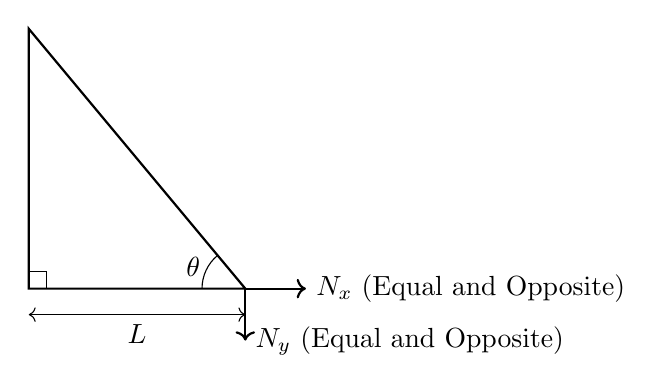
\begin{tikzpicture}[scale=1.1]
        % Right triangle
        \draw[thick] (0,3) -- (0,0) -- (2.5,0) -- cycle;
        
        % Right angle symbol
        \draw (0,0.2) -- (0.2,0.2) -- (0.2,0);
        
        % Length L label
        \draw[<->] (0,-0.3) -- (2.5,-0.3) node[midway, below] {$L$};
        
        % Angle theta
        \draw (2.5,0) ++(180:0.5) arc (180:130:0.5);
        \node at (1.9, 0.25) {$\theta$};
    
        
        % Forces at bottom right
        \draw[->, thick] (2.5,0) -- (3.2,0) node[right] {$N_x$ (Equal and Opposite)};
        \draw[->, thick] (2.5,0) -- (2.5,-0.6) node[right] {$N_y$  (Equal and Opposite)};
    \end{tikzpicture}
    \end{minipage}%
    \hfill
    \begin{minipage}[t]{0.59\textwidth}
    \vspace{0pt}
    At the point of contact,\\
    let there be $N_y$ in vertical and $N_x$ in horizontal.
    
    \vspace{0.5em}
    \noindent At the bottom edge hinge,
    \[
    \frac{\rho L^2 g}{2} = N_y L
     \implies N_y = \frac{\rho L g}{2}
    \]
    \end{minipage}
    
    \vspace{0.5em}
    \noindent Now, about top hinge:
    \begin{align*}
    N_y L + \frac{\rho L}{\cos\theta} g \frac{L}{2} &= N_x \tan\theta L \\[6pt]
    \frac{\rho L g}{2} + \frac{\rho L g}{2\cos\theta} &= N_x \tan\theta \\[6pt]
    \implies \frac{\rho L g}{2} \cot\theta \left[ 1 + \frac{1}{\cos\theta} \right] &= N_x
    \end{align*}
    \begin{align*}
    F_{HY} &= N_y + \frac{\rho L}{\cos\theta} g \\[8pt]
    F_{HY} &= \rho L g \left[ \frac{1}{2} + \frac{1}{\cos\theta} \right] = \frac{\rho L g}{2} \left[ 1 + \frac{2}{\cos\theta} \right] = \frac{\rho L g}{2} \left[ 1 + 2 \sec\theta \right] \\[8pt]
    F_{HX} &= \frac{\rho L g}{2} \cot\theta \left[ 1 + \frac{1}{\cos\theta} \right] = \frac{\rho L g}{2} \left[ \cot\theta + \frac{1}{\sin\theta} \right]
    \end{align*}
    
    \vspace{1em}
    \noindent
    \textbf{Now,}
    
    \vspace{0.5em}
    \noindent
    \begin{minipage}[t]{0.48\textwidth}
    \textbf{at } $\mathbf{\theta = 0}$
    \begin{align*}
    \cot\theta &\to \infty \\
    \implies F_{HX} &\to \infty \\
    \implies F_H &\to \infty
    \end{align*}
    \end{minipage}%
    \hfill
    \begin{minipage}[t]{0.48\textwidth}
    \textbf{at } $\mathbf{\theta = \frac{\pi}{2}}$
    \begin{align*}
    \sec\theta &\to \infty \\
    F_{HY} &\to \infty \\
    \implies F_H &\to \infty
    \end{align*}
    \end{minipage}
\end{solution}
\begin{problem}
    \begin{minipage}[t]{0.68\textwidth}
      \noindent
    A stick leans at an angle $\theta$ to the horizontal, resting tangentially against a circle of radius $R$ that stands on flat ground. If the system is to remain at rest, show that the coefficient of friction:
    
    \vspace{0.5em}
    \begin{itemize}
        \item[(a)] between the stick and the circle must satisfy
        \begin{equation*}
            \mu \ge \frac{\sin\theta}{1 + \cos\theta}. \hfill (1.14)
        \end{equation*}
        \item[(b)] between the stick and the ground must satisfy$^6$
        \begin{equation*}
            \mu \ge \frac{\sin\theta \cos\theta}{(1 + \cos\theta)(2 - \cos\theta)}. \hfill (1.15)
        \end{equation*}
    \end{itemize}
    \end{minipage}%
    \hfill
    \begin{minipage}[t]{0.28\textwidth}
    \vspace{0pt}
    \centering
    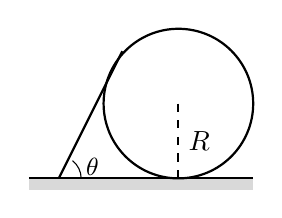
\begin{tikzpicture}[scale=0.95]
        % Ground shading
        \fill[gray!30] (-0.2, -0.15) rectangle (2.8, 0);
        \draw[thick] (-0.2, 0) -- (2.8, 0);
        
        % Circle
        \draw[thick] (1.8, 1.0) circle (1.0);
        
        % Radius R (dashed)
        \draw[dashed, thick] (1.8, 1.0) -- (1.8, 0) node[midway, right] {$R$};
        
        % Tangent stick
        \draw[thick] (0.2, 0) -- (1.05, 1.7);
        
        % Angle theta
        \draw (0.5, 0) arc (0:52:0.3);
        \node at (0.65, 0.15) {\small $\theta$};
    \end{tikzpicture}
    \captionof{figure}{}
    \vspace{0.5em}
    \end{minipage}
\end{problem}
\begin{solution}
    \noindent
    \begin{minipage}[t]{0.38\textwidth}
    \vspace{0pt}
    \centering
    \textbf{Circle}
    
    \vspace{0.5em}
    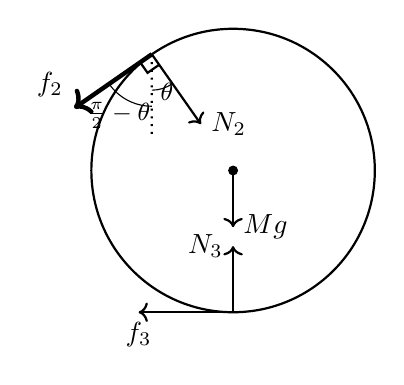
\begin{tikzpicture}[scale=1.2]
        % Circle
        \draw[thick] (0,0) circle (1.5);
        
        % Center dot and gravity Mg
        \fill (0,0) circle (1.5pt);
        \draw[->, thick] (0,0) -- (0,-0.6) node[right] {$Mg$};
        
        % Bottom contact forces
        \draw[->, thick] (0,-1.5) -- (0,-0.8) node[left] {$N_3$};
        \draw[->, thick] (0,-1.5) -- (-1.0,-1.5) node[below] {$f_3$};
        
        % Contact point at top-left
        \coordinate (P) at (-0.86, 1.23);
        \coordinate (N2) at ($(P) + (0.52, -0.74)$);
        \coordinate (F2) at ($(P) + (-0.82, -0.57)$);
        \coordinate (V)  at ($(P) + (0, -0.9)$);
        
        % Force vectors at contact point
        \draw[->, ultra thick] (P) -- (F2) node[above left] {$f_2$};
        \draw[->, thick] (P) -- (N2) node[right] {$N_2$};
        
        % Dotted vertical reference line
        \draw[thick, dotted] (P) -- (V);
        
        % Right angle symbol between f2 and N2
        \draw[thick] ($(P)!0.15!(F2)$) -- ($($(P)!0.15!(F2)$) + ($(P)!0.15!(N2)$) - (P)$) -- ($(P)!0.15!(N2)$);
        
        % Angle arcs and labels
        \draw (P) ++(270:0.38) arc (270:305:0.38);
        \node at ($(P) + (0.16, -0.40)$) {\small $\theta$};
        
        \draw (P) ++(215:0.55) arc (215:270:0.55);
        \node at ($(P) + (-0.35, -0.65)$) {\small $\frac{\pi}{2}-\theta$};
    \end{tikzpicture}
    \end{minipage}%
    \hfill
    \begin{minipage}[t]{0.59\textwidth}
    \vspace{0pt}
    \noindent
    To balance torque,
    \[
    f_2 = f_3
    \]
    
    \noindent
    Balancing horizontally,
    \begin{align*}
    f_2 \cos\theta + f_3 &= N_2 \sin\theta \\
    \implies f_2 [\cos\theta + 1] &= N_2 \sin\theta \\
    \implies f_2 &= \frac{N_2 \sin\theta}{1 + \cos\theta}
    \end{align*}
    
    \vspace{0.5em}
    \noindent
    Now,
    \begin{align*}
    \mu_2 N_2 &\ge f_2 \\
    \implies \mu_2 N_2 &\ge \frac{N_2 \sin\theta}{1 + \cos\theta} \\[6pt]
    \implies \mu_2 &\ge \frac{\sin\theta}{1 + \cos\theta}
    \end{align*}
    \end{minipage}
    \noindent
    \begin{minipage}[t]{0.38\textwidth}
    \vspace{0pt}
    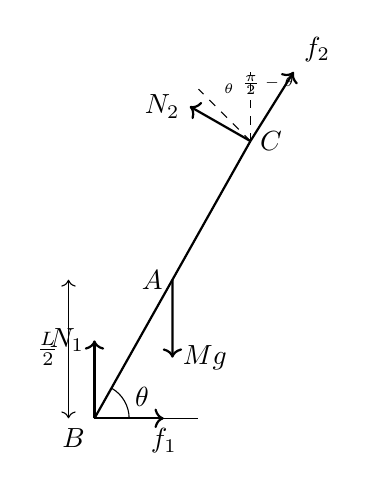
\begin{tikzpicture}[scale=1.1]
        % Coordinates
        \coordinate (B) at (0,0);
        \coordinate (C) at (1.8,3.2);
        \coordinate (A) at (0.9,1.6);
        
        % Rod
        \draw[thick] (B) -- (C);
        
        % Points
        \node[below left] at (B) {$B$};
        \node[left] at (A) {$A$};
        \node[right] at (C) {$C$};
        
        % Ground line & angle theta at B
        \draw (B) -- (1.2,0);
        \draw (0.4,0) arc (0:60:0.4);
        \node at (0.55,0.25) {$\theta$};
        
        % Forces at B
        \draw[->, thick] (B) -- (0,0.9) node[left] {$N_1$};
        \draw[->, thick] (B) -- (0.8,0) node[below] {$f_1$};
        
        % Length L/2 dimension
        \draw[<->] (-0.3,0) -- (-0.3,1.6) node[midway, left] {$\frac{L}{2}$};
        
        % Force at A (Mg)
        \draw[->, thick] (A) -- (0.9,0.7) node[right] {$Mg$};
        
        % Forces at C
        \draw[->, thick] (C) -- ++(-0.7,0.4) node[left] {$N_2$};
        \draw[->, thick] (C) -- ++(0.5,0.8) node[above right] {$f_2$};
        
        % Angles at C
        \draw[dashed] (C) -- ++(0,0.8);
        \draw[dashed] (C) -- ++(-0.6,0.6);
        \node at ($(C)+(-0.25,0.6)$) {\tiny $\theta$};
        \node at ($(C)+(0.2,0.65)$) {\tiny $\frac{\pi}{2}-\theta$};
    \end{tikzpicture}
    \end{minipage}%
    \hfill
    \begin{minipage}[t]{0.59\textwidth}
    \vspace{0pt}
    \textbf{About ground,}
    \[
    N_2 L = \frac{Mg L}{2} \cos\theta \implies N_2 = \frac{Mg}{2} \cos\theta
    \]
    
    \vspace{0.5em}
    \textbf{At $C$,}
    \begin{align*}
    N_2 \sin\theta - f_2 \cos\theta &= F_{\text{HORI}} \\
    \implies F_{\text{HORI}} &\le N_2 \sin\theta - \mu_2 N_2 \cos\theta \\
    &\le N_2 \left[ \sin\theta - \mu_2 \cos\theta \right] \\
    &\le N_2 \left[ 1 - \frac{\sin\theta \cos\theta}{1 + \cos\theta} \right] \\
    &\le N_2 \left[ \frac{\sin\theta}{1 + \cos\theta} \right]
    \end{align*}
    \[
    \therefore F_{\text{HORI}} \ge 0 \implies f_1 \text{ must act inward}
    \]
    \end{minipage}
    
    \vspace{1.5em}
    \noindent
    \textbf{About $C$,}
    \begin{align*}
    f_1 L \sin\theta + \frac{Mg L}{2} \cos\theta &= N_1 L \cos\theta \\
    \implies f_1 \sin\theta + \frac{Mg}{2} \cos\theta &= N_1 \cos\theta \\
    \implies f_1 \tan\theta + \frac{Mg}{2} &= N_1
    \end{align*}
    
    \vspace{1em}
    \noindent
    \textbf{Balancing weight}
    \begin{align*}
    Mg &= N_1 + N_2 \cos\theta + N_2 \mu_2 \sin\theta \\
    &= N_1 + N_2 \cos\theta + \frac{N_2 \sin^2\theta}{1 + \cos\theta} \quad \left[ \text{Now, } \frac{\sin^2\theta}{1 + \cos\theta} = 1 - \cos\theta \right] \\
    &= N_1 + N_2 \cos\theta + N_2 (1 - \cos\theta) \\
    &= N_1 + N_2 \\[6pt]
    \implies Mg &= \frac{Mg}{2} \cos\theta + N_1 \\
    \implies \frac{Mg}{2} \left[ 2 - \cos\theta \right] &= N_1 \\
    \implies \frac{N_1}{2 - \cos\theta} &= \frac{Mg}{2}
    \end{align*}
    \begin{align*}
    \therefore f_1 \tan\theta &= N_1 - \frac{N_1}{2 - \cos\theta} \\[8pt]
    N_1 \mu_1 \tan\theta &\ge N_1 \left[ 1 - \frac{1}{2 - \cos\theta} \right] \\[8pt]
    \mu_1 &\ge \frac{1}{\tan\theta} \left[ 1 - \frac{1}{2 - \cos\theta} \right] \\[8pt]
    \mu_1 &\ge \frac{\cos\theta (1 - \cos\theta)}{\sin\theta (2 - \cos\theta)} \\[8pt]
    \implies \mu_1 &\ge \frac{\cos\theta \sin\theta}{(1 + \cos\theta)(2 - \cos\theta)}
    \end{align*}
\end{solution}
\end{document}